%\documentclass{beamer}
\documentclass[serif]{beamer}
%--------------------------------------------------------------------------------------------------------------------------------------------
%----------------------------------------------------------PACKAGES---------------------------------------------------------------------
%--------------------------------------------------------------------------------------------------------------------------------------------
%\usepackage[T1]{fontenc}
%\usepackage{concmath}
\usepackage{beamerthemesplit}
\usepackage[utf8x]{inputenc}
\usepackage[italian, UKenglish]{babel}
%\usepackage [pdftex]{graphicx}
\usepackage [bf, small]{caption}
%\usepackage {caption}
\usepackage{mathtools}
\usepackage{tikz}
\usepackage{amsmath}
\usepackage{amsthm}
\usepackage{amssymb}
\usepackage{fancyhdr}
\usepackage{wrapfig}
\usepackage{subfigure}
\usepackage{newlfont}
\usepackage{hyperref}
\usepackage{verbatim}
\usepackage{leftidx}
\usepackage{mathabx}
%--------------------------------------------------------------------------------------------------------------------------------------------
%--------------------------------------------------NEW COMMANDS---------------------------------------------------------------------
%--------------------------------------------------------------------------------------------------------------------------------------------
%\usecolortheme[named=red]{structure}
\makeatletter
\newcommand\mathcircledred[1]{%
  \mathpalette\@mathcircledred{#1}%
}
\newcommand\@mathcircledred[2]{%
  \tikz[baseline=(math.base)] \node[draw,circle,inner sep=1pt, red] (math) {$\m@th#1#2$};%
}
\makeatother

\makeatletter
\newcommand\mathcircledgreen[1]{%
  \mathpalette\@mathcircledgreen{#1}%
}
\newcommand\@mathcircledgreen[2]{%
  \tikz[baseline=(math.base)] \node[draw,circle,inner sep=1pt, green] (math) {$\m@th#1#2$};%
}
\makeatother
%--------------------------------------------------------------------------------------------------------------------------------------------
%---------------------------------------------------------COMMANDS---------------------------------------------------------------------
%--------------------------------------------------------------------------------------------------------------------------------------------
%\theoremstyle{plain}
\theoremstyle{definition}
\newtheorem*{defin}{Definition}
\newtheorem*{obs}{Observation}
\newtheorem*{theor}{Theorem}
\newtheorem*{rec}{Recall}
\newtheorem*{prop}{Proposition}
\newtheorem*{no}{Notation}
\newtheorem*{pr}{Problem}
\newtheorem*{cor}{Corollary}
\newtheorem*{idea}{Idea}
%--------------------------------------------------------------------------------------------------------------------------------------------
%------------------------------------------------------------TITLE-------------------------------------------------------------------------
%--------------------------------------------------------------------------------------------------------------------------------------------
\title[The Heisenberg... what?] 
{The Heisenberg... what?}
%\subtitle
%{Include Only If Paper Has a Subtitle}
\author%[Giovanni Canarecci] % (optional, use only with lots of authors)
{Giovanni Canarecci}
% - Give the names in the same order as the appear in the paper.
% - Use the \inst{?} command only if the authors have different
%   affiliation.
\institute[University of Helsinki] % (optional, but mostly needed)
{
  Department of Mathematics and Statistics\\
  University of Helsinki
}
% - Use the \inst command only if there are several affiliations.
% - Keep it simple, no one is interested in your street address.

\date[25/05/2018] % (optional, should be abbreviation of conference name)
{25/05/2018}
% - Either use conference name or its abbreviation.
% - Not really informative to the audience, more for people (including
%   yourself) who are reading the slides online
% If you have a file called "university-logo-filename.xxx", where xxx is a graphic format that can be processed by latex or pdflatex, resp., then you can add a logo as follows:
\pgfdeclareimage[height=1cm]{university-logo}{HY_logo}
\logo{\pgfuseimage{university-logo}}
%
% Delete this, if you do not want the table of contents to pop up at
% the beginning of each subsection:
%\AtBeginSubsection[]
%{
%  \begin{frame}<beamer>{Content}
%    \tableofcontents[currentsection,currentsubsection]
%  \end{frame}
%}
%
% If you wish to uncover everything in a step-wise fashion, uncomment
% the following command: 
%\beamerdefaultoverlayspecification{<+->}
% PER FAR APPARIRE LE SCRITTE A POCO A POCO
%--------------------------------------------------------------------------------------------------------------------------------------------
%----------------------------------------------------------DOCUMENT---------------------------------------------------------------------
%--------------------------------------------------------------------------------------------------------------------------------------------
\begin{document}


%\frame{\titlepage}
\begin{frame}
  \titlepage
\end{frame}

%------------------------------------------------------------------------------------------------------------------------------

%\section[CONTENUTI]{}
%\begin{frame}{Contents}
%  \tableofcontents
  % You might wish to add the option [pausesections]
%\end{frame}

%------------------------------------------------------------------------------------------------------------------------------

\section{The Heisenberg Group...}

\begin{frame}{}
The first Heisenberg Group is a three dimensional manifold
$$\mathbb{H}^1= ( \mathbb{R}^3, g_{cc} )$$
that carries a natural intrinsic metric $g_{cc}$ called the Carnot–Carathéodory metric.
\vspace{\baselineskip}
This metric gives an orthonormal basis for the tangent space as
 $$
\begin{cases}
X=\partial_x-\frac{1}{2}y\partial_t\\
Y=\partial_y+\frac{1}{2}x\partial_t\\
T=\partial_t
\end{cases}
 $$
\end{frame}

%------------------------------------------------------------------------------------------------------------------------------

\section{... in pictures}
\begin{frame}{}
\begin{figure}
\centering
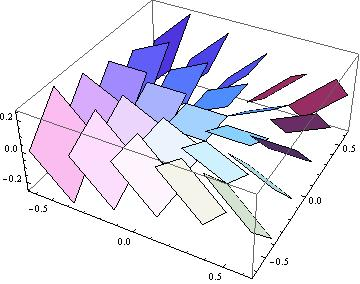
\includegraphics[width= 10 cm]{Distribution1.jpg}
\end{figure}
\end{frame}

%------------------------------------------------------------------------------------------------------------------------------

\begin{frame}{}
\begin{figure}[!ht]
\centering
{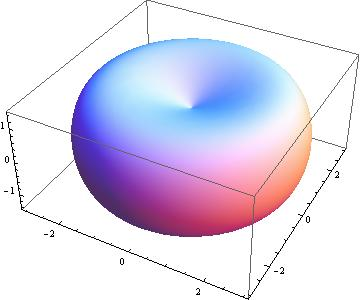
\includegraphics[width=5.3 cm]{CCSphere.jpg}}
{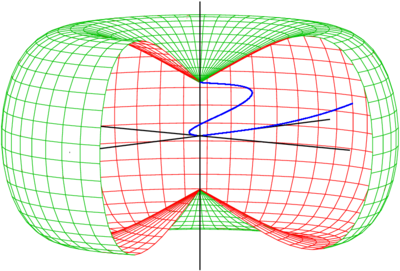
\includegraphics[width=5.3 cm]{O6NE6.png}}
\end{figure}
%\begin{figure}
%\centering
%\includegraphics[width= 10 cm]{Plateau_problem_02.jpg}
%\end{figure}
\end{frame}

%------------------------------------------------------------------------------------------------------------------------------

\subsection{}
\begin{frame}
\begin{center}
\huge{Kiitos paljon!}\\
\huge{Thank you!}\\
\huge{Grazie mille!}
\end{center}
\end{frame}

\end{document}%%%%%%%%%%%%
%------------------------------------------------------------------------------------------------------------------------------
%------------------------------------------------------------------------------------------------------------------------------
%------------------------------------------------------------------------------------------------------------------------------
%------------------------------------------------------------------------------------------------------------------------------
%------------------------------------------------------------------------------------------------------------------------------